\documentclass{article}
\usepackage[utf8]{inputenc}
\usepackage{graphicx}
\usepackage{amsmath}
\usepackage{amssymb}
\usepackage{amsthm}
\usepackage{bm}

\title{Computational Physics (physics760)\\Exercise 6}
\author{Ajay S. Sakthivasan, Dongjin Suh}
\date{December 9, 2022}

\begin{document}

\maketitle

\begin{enumerate}

\item   \textbf{Correlator Bias}\\
As discussed in the lecture, the algorithm may not explore all spin configurations for large ($\gg J_c$) value of $J$. The algorithm might settle for one particular spin configuration, either almost all spin-up or almost all spin-down, in which case the correlator will always be close to $1$. This means that there is no bias in the Correlator, since we expect for large values of $J$, the correlation to be close to $1$.

\item \textbf{Correlator ($r = 0$)}\\
If $r=0$, we are calculating the correlation o each spin site with itself. Since, each spin can either up or down, the product will always be $1$. Dividing by the total number of sites, we get $C_0 = 1$.

\item \textbf{Correlator as convolution}\\
We proceeded to implement the correlator as a convolution. This can be found in the file \texttt{corr.py}. For $r=0$, we obtain the expected value of $1$.

\item \textbf{Behaviour of $C$ for different $N$}\\
Due to time constraints, we evaluated the behaviour of $C$ at the critical value for the values of $N = 3, 5, 7, 9, 11$, for $1000$ sweeps over the entire lattice. The obtained plots, \ref{fig:CN}, are given below. Note that the $x$-axis contains the values of $r$ and the $y$-axis has the values of the $r$-correlator. We aim to update this to $20000$ sweeps and up to a lattice size of $23$ for the next submission.
\begin{figure}
    \centering
    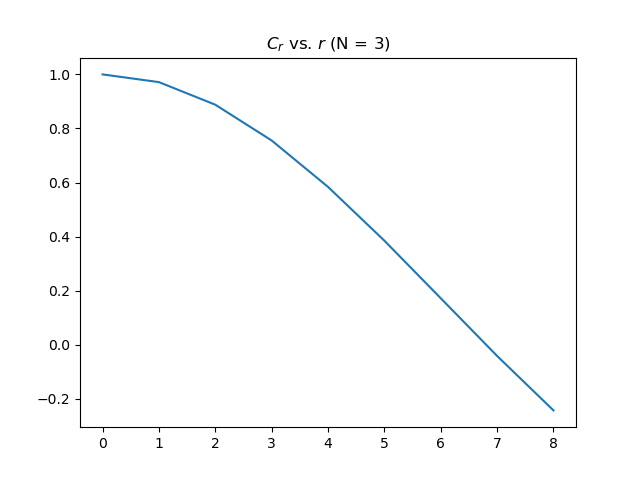
\includegraphics[width=.4\linewidth]{N3.png}
    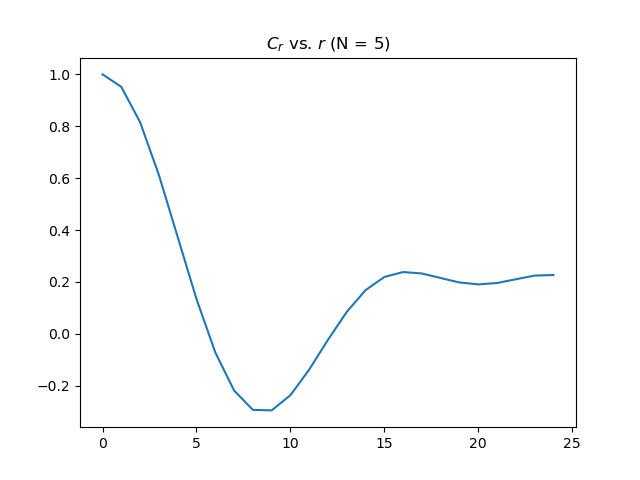
\includegraphics[width=.4\linewidth]{N5.png}
    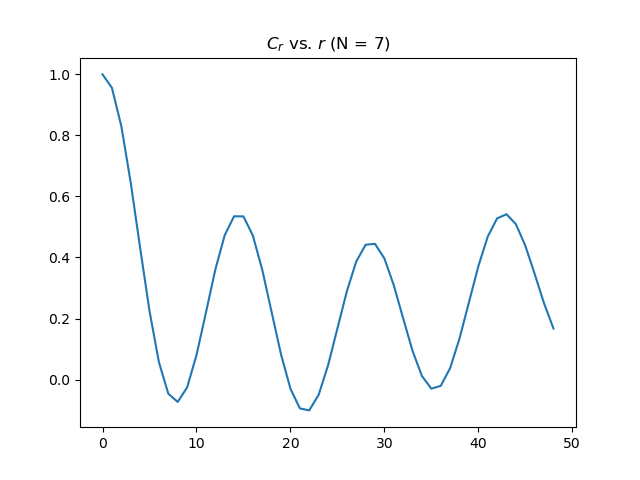
\includegraphics[width=.4\linewidth]{N7.png}
    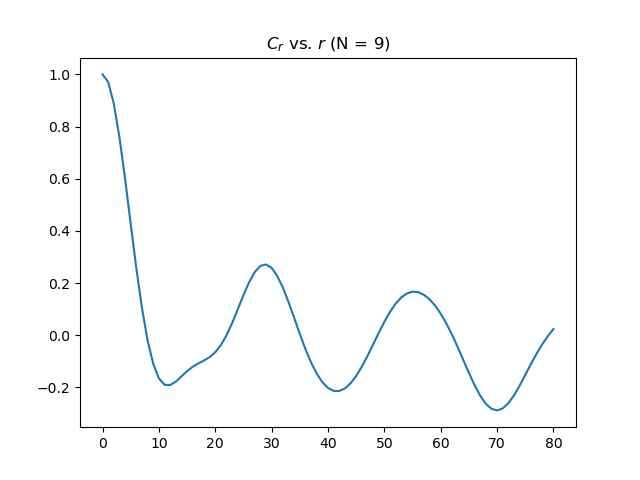
\includegraphics[width=.4\linewidth]{N9.png}
    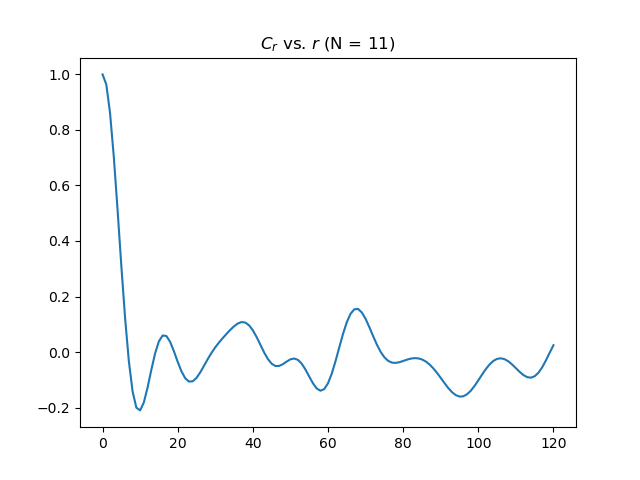
\includegraphics[width=.4\linewidth]{N11.png}
    \caption{Behaviour of $C$ for different $N$. $x$-axis: $r$-values; $y$-axis: Correlator}
    \label{fig:CN}
\end{figure}

\end{enumerate}
\end{document}
